\subsection{YOLOv8}

Вышедшая в январе 2023 года YOLOv8 является последней версией семейства моделей детектирования и сегментации YOLO на момент написания работы. В ней все еще используются многие компоненты архитектуры YOLOv5 такие, как Cross-Stage-Partial Network (CSP), метод слияния признаков PAN-FPN и модуль Spatial Pyramid Pooling - Fast (SPPF), однако присутствуют и следующие изменения \cite{6-1}:

\begin{itemize}

    \item Представленная новая модель SOTA, содержащая P5 640 и P6 1280 блоки обнаружения объектов, позволяющие лучше работать с объектами разных размеров на изображениях с разрешениями 640x640 и 1280x1280, а также модель сегментации YOLACT \cite{6-2}.

    \item Используемый в компоненте Head метод разделения частей, ответственных за детектирование и классификацию \cite{6-3}.

    \item Новая функция потерь для регрессии CIOU Loss + DFL (Distribution Focal Loss) \cite{6-4}:

    \begin{equation}
        DFL(s_i, s_{i+1}) = -((y_{i+1}-y)\log(s_i) + (y-y_i)\log(s_{i+1})),
    \end{equation}

    \noindent где $s_i$ и $s_{i+1}$ -- выходы сигмоиды, $y_i$ и $y_{i+1}$ -- интервальные порядки, а $y$ -- метка.

    \item Новая функция потерь для классификации VFL (Varifocal Loss) \cite{6-5}:

    \begin{equation}
        VFL(p, q) = 
        \begin{cases}
            -q(q\log(p)+(1-q)\log(1-p)), \quad q>0 \\
            -\alpha p^{\gamma} \log(1-p), \quad q=0
        \end{cases},
    \end{equation}

    \noindent где $p$ -- получен IoU-Aware Classification Score (IACS), $q$ -- целевая IoU оценка.

    \item Ancor-Free метод вместо Anchor-Base.
    
\end{itemize}

Компонента Backbone осталась практически той же, что и у YOLOv5, однако модуль C3 заменен модулем C2f для получения более обширной информации о градиентном потоке при сохранении легковесности модели. Модуль C2f появился исходя из идеи ELAN (Efficient Layer Aggregation Network) в модели YOLOv7 \cite{6-6}, став его объединением с модулем C3.

В компоненте Neck все еще используется PAN-FPN, улучшающий слияние и использование информации о признаках с различных слоев при различных масштабах. В компоненте Head происходит замена Coupled-Head на Decoupled-Head \cite{6-7}. Полная схема структуры модели представлена на Рис. \ref{img:6-1}.

Присваивание меток является одной из важнейших частей детектирования объектов. В версии YOLOv5 в качестве метода присваивания использовался MaxIoU, однако прямое использование отношения длин сторон может достичь тех же результатов, потому стал применяться TaskAligned. Для этого была разработана новая метрика, использующая комбинацию оценки классификации и IoU для вычисления степени совпадения следующим образом:

\begin{equation}
    t = s^{\alpha} \times u^{\beta},
\end{equation}

\noindent где $s$ -- точность классификации, $u$ -- значение IoU, а $\alpha$ и $\beta$ -- весовые гиперпараметры.

\begin{figure}[ht]
    \centering
    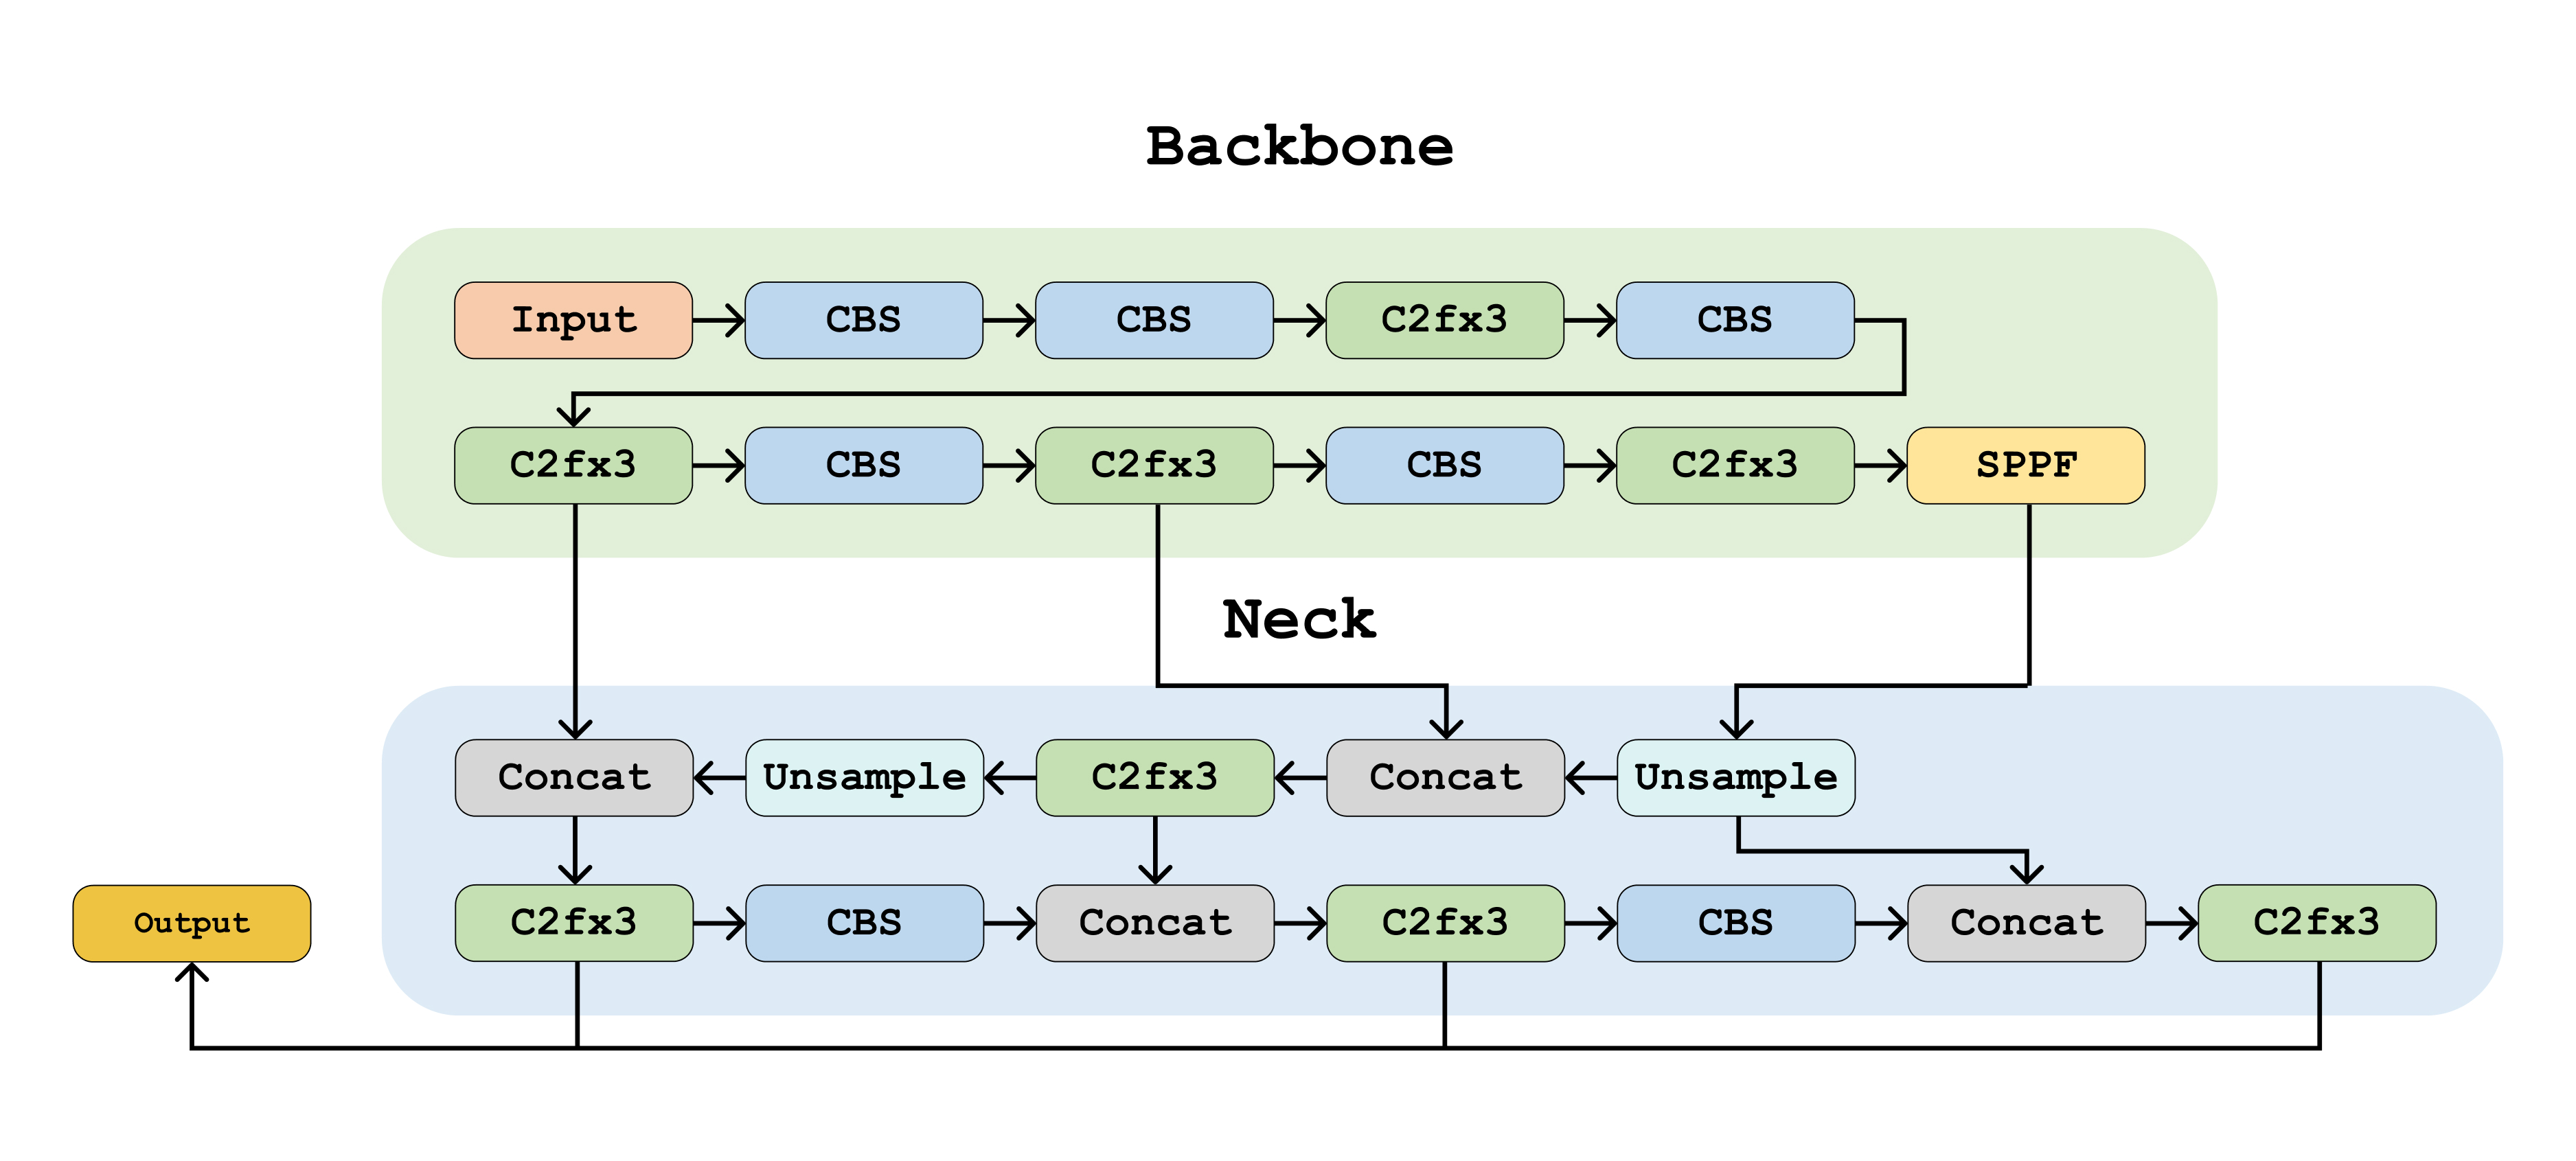
\includegraphics[width=0.85\textwidth]{6-1}
    \caption{Схема структуры модели YOLOv8}
    \label{img:6-1}
\end{figure}

Одними из главных нововведений YOLOv8, представляющими интерес в данной работе, являются встроенные алгоритмы трекинга -- BoT-SORT \cite{6-8} и ByteTrack \cite{6-9}. 
